%#################################################################################
	%beginning
	\documentclass[12pt, a4paper]{scrreprt}
		
	%Worttrennung Deutsch
	\usepackage[ngerman]{babel}
	
	%Trennung von Umlauten
	\usepackage{fontspec}
	
	%Zeilenabstand
	\usepackage{setspace}
	
	%Moderne Schrift
	\usepackage{lmodern}
	\setmainfont[Ligatures=TeX]{Arial}
	\renewcommand*\familydefault{\sfdefault}
	
	%Bilder
	\usepackage{graphicx}
	\usepackage{float}
	
	%Quellen
	\usepackage[backend=bibtex,sorting=ynt,useauthor=true,]{biblatex}
		
	%Formeln
	\usepackage{amsmath}
		
	%Clever Reference
	\usepackage{hyperref}
	\usepackage[capitalise]{cleveref}
	
	%Quellcode
	\usepackage{listings}
	\usepackage{xcolor}
	\lstset{language=python,
		basicstyle=\footnotesize\ttfamily,
		keywordstyle=\color{blue},
		stringstyle=\color{green},
		commentstyle=\color{red}
		}
	
	%Einrückungen
	\usepackage{parskip}
	
	%Variablen
	\newcommand{\Titel}{Information Retrieval}
	\newcommand{\Autor}{Jesse-Jermaine Richter, Jonas Seng}
	\newcommand{\TotPages}{35}
	
	%Literaturverzeichnis
	\bibliography{lit.bib}
	
	%Inhaltsverzeicnis
	\setcounter{tocdepth}{1}
	
	%Multiline Kommentare
	\usepackage{verbatim}
	
	%Header/Footer
	\usepackage{totpages}
	\usepackage[includeheadfoot, left=2.5cm, top=1.5cm, bottom=1cm]{geometry}
	
	\usepackage{fancyhdr}
	
	\lhead{\nouppercase{\leftmark}}
	\chead{}
	\rhead{\nouppercase{\rightmark}}
	\lfoot{\Titel}
	\cfoot{}
	\rfoot{Seite \thepage\ von \TotPages}
	\renewcommand{\headrulewidth}{0.2pt}
	
	\fancypagestyle{plain}{
		\fancyhf{}
		\renewcommand{\headrulewidth}{0pt}
		\lfoot{\Titel}
		\rfoot{Seite \thepage\ von \TotPages}
	}

	\usepackage{afterpage}
	
	\newcommand\blankpage{%
		\null
		\thispagestyle{empty}%
		\addtocounter{page}{-1}%
		\newpage}
	
	\newtheorem{defi}{Definition}[chapter]
	
%#################################################################################
%#################################################################################

%DOCUMENT BEGIN
\begin{document}	
%---------------------------------------------------------------------------------
		\begin{titlepage}
		
		\centering
		{\Large\bfseries \Titel \par}
		\vspace{2cm}
		Seminararbeit \par
		\vspace{3cm}
		
		des Studienganges Angewandte Informatik \par
		an der Dualen Hochschule Baden-Württemberg Mannheim \par
		\vspace{3cm}
		
		von \par
		\vspace{0.5cm}
		{\itshape \Autor \par}
		\vspace{2cm}
		27.08.2018 \par
		
		\vspace{6.5cm}
		\begin{tabular}{llll}
			Matrikelnummer, Kurs: & & & 8787549/1980179, TINF16AIBI\\
			Ausbildungsfirma: & & & DZ BANK AG, Frankfurt\\
			Betreuer der Ausarbeitung: & & & Herr Prof. Dr. Karl Stroetmann
		\end{tabular}
	\end{titlepage}
	\thispagestyle{empty}
%---------------------------------------------------------------------------------			
	\section*{Erklärung}
	Ich versichere hiermit, dass ich meine Projektarbeit mit dem Thema: \glqq\Titel\grqq{ }selbstständig verfasst und keine anderen als die angegebenen Quellen und Hilfsmittel benutzt habe.

Ich versichere zudem, dass die eingereichte elektronische Fassung mit der gedruckten Fassung übereinstimmt.\\\\\\\\\\\\
\renewcommand{\arraystretch}{0.5}
\begin{tabular}{l@{\hspace{4cm}}l@{\hspace{4cm}}l@{\hspace{4cm}}l}
	\cline{1-1} \cline{3-3} \\
	Ort, Datum && Unterschrift & \\
\end{tabular}
	\thispagestyle{empty}
	\newpage
%---------------------------------------------------------------------------------
	\begin{abstract}
		\begin{spacing}{1,6}
	In diesem Praxisbericht wird das Thema \glqq\Titel\grqq\ behandelt. Hierbei soll der Leser ein Überblick bekommen, was Monitoring ist, welche Vorteile es birgt, ob es sich um ein notwendiges Werkzeug zur verlässlichen Bereitstellung von IT-Sevices handelt und ob es Alternativen gibt. Außerdem wird ein praktischer Teil präsentiert, in welchem ein Quellcode gezeigt wird, der die Teilimplementierung eines Monitoring-Systems widerspiegelt. Hier werden Daten für eine Statusmail verarbeitet und visualisiert.
	
	This practical report deals with the topic \glqq\Titel\grqq . The reader should get an overview of what monitoring is, what advantages it offers, whether it is a necessary tool for reliable provision of IT services and whether there are alternatives. In addition, a practical part is presented in which a source code is shown that reflects the partial implementation of a monitoring system. Data for a status mail is processed and visualized here.
\end{spacing}

	\end{abstract}
	\afterpage{\blankpage}
%---------------------------------------------------------------------------------			
	\tableofcontents
	\thispagestyle{empty}
%---------------------------------------------------------------------------------			
	%Abbildungsverzeichnis
	\listoffigures
	\thispagestyle{empty}
%---------------------------------------------------------------------------------			
	\chapter*{Abkürzungstabelle}
	\label{abkürzung}
	\renewcommand{\arraystretch}{1.5}
\begin{center}
	\begin{tabular}{|l|l|}\hline
		\multicolumn{1}{|c|}{\textbf{Abkürzung:}} & \multicolumn{1}{c|}{\textbf{Bedeutung:}} \\ \hline
		ASCII & American Standard Code for Information Interchange \\ \hline
		DF & Document Frequency \\ \hline
		IDF & Inverse Document Frequency \\ \hline
		IR & Information Retrieval \\ \hline
		PDF & Portable Document Format \\ \hline
		TF & Term Frequency \\ \hline
		TF-IDF & TF-IDF-Maß \\ \hline
	\end{tabular}
\end{center}

	\thispagestyle{empty}
	\pagestyle{fancy}
	\begin{spacing}{1.5}	
%---------------------------------------------------------------------------------
		\chapter{Einleitung}\pagenumbering{arabic}
		\label{einleitung}
		\section{Was ist Information-Retrieval?}
Information-Retrieval (IR) beschreibt das Bereitstellen spezieller Informationen aus einer großen und unsortierten Datenmengen. Dieses Themengebiet fällt unter Informatik, Informationswissenschaften sowie Computerlinguistik und ist ein wesentlicher Bestandteil von Suchmaschinen wie zum Beispiel Google.
\\
Das Thema besitzt bereits seit einigen Jahren eine hohe, aber dennoch steigende Relevanz. Die Gründe der hohen Relevanz von IR liegen vor allem beim Einsatz von Suchmaschinen. Diese sind in Zeiten des Internets die wohl wichtigste Form der Informationsbeschaffung. Aufgrund der immer schneller steigenden Informationsmengen wird das Thema künftig weiter an Relevanz gewinnen. Unternehmen und Privatanwender wird eine immer wachsende Menge von Informationen zugänglich, die organisiert werden muss, damit relevante bzw. spezifisch gesuchte Informationen jederzeit und ohne Verzögerung gefunden werden.
\\
Um das Ziel der Bereitstellung von Informationen gewährleisten zu können, wird erst eine Durchsuchung und Gewichtung sämtlicher Informationen bzw. Dokumente, die später gefunden werden sollen, durchgeführt. Das zentrale Objekt der Informationsrückgewinnung stellt der invertierte Index dar, dessen Aufbau und Funktionsweise in den nächsten Kapiteln ausführlich erläutert wird. Im Verlauf dieser Arbeit wird die Komprimierung des Indexes sowie das TF-IDF-Maß, welches zur Beurteilung der Relevanz eines Dokumentes genutzt wird, im Fokus stehen.
\\
Die theoretischen Hintergründe des invertierten Index, der Komprimierung und des TF-IDF-Maß werden durch eine Beispiel-Implementierung einer lokalen Suchmaschine in Programmiersprache Python veranschaulicht.

\section{Ziel der Arbeit}
Ziel der Arbeit ist es, ein grundlegendes Verständnis des Themenkomplexes Information-Retrieval zu vermitteln. Das umfasst auch die theoretischen Hintergründe, die für die später vorgestellten Beispielimplementierungen notwendig sind.
\\
Die Beispielimplementierung soll hauptsächlich die folgenden Themengebiete umfassen:\\
\begin{itemize}
	\item Aufbau eines invertierten Indexes
	\item Approximierende Beurteilung der Relevanz eines gefundenen Dokuments mittels tf-idf
	\item Komprimierung des invertierten Indexes
\end{itemize}
Die in dieser Arbeit vorgestellte Implementierung hat nicht den Anspruch auf eine hohe Performance, vielmehr dient diese dem Zwecke der praxisnahen Veranschaulichung der Funktionsweise von IR-Systemen.

\section{Stand der Forschung}
Dieser Abschnitt umreißt kurz den aktuellen Stand der Forschung. Dazu werden zwei Modelle von Information Retrieval knapp beschrieben, die für die Entwicklung einer lokalen Suchmaschine, von Bedeutung sind. Es wird jedoch nur auf ein Modell im Verlauf dieser Arbeit eingegangen.
\\

\subsection{Vector Space Model}
Das Vector Space Model, zu deutsch Vektorraummodell, repräsentiert Dokumente und Anfragen als hochdimensionale, metrische Vektoren \cite{VR_Retrieval}.
Der Anfrage-Vektor wird beim Retrieval-Prozess mit den Dokumenten-Vektoren verglichen. Dabei werden jedoch nur Dokumente betrachtet, welche mit der Anfrage in Verbindung stehen \cite{klass_IR}. Welche Dokumente betrachtet werden, wird mithilfe des invertierten Index ermittelt.
\\
Es gibt verschiedene Maße, mit denen die Vektoren miteinander verglichen werden. Der einfachste Ansatz besteht darin, den Abstand zu berechnen, jedoch ist dies kein sehr gutes Maß. Besser und weit verbreitet ist deshalb das Cosinus-Maß (oder Kosinus-Ähnlichkeit), welches den Winkel zwischen Anfrage-Vektor und Dokumenten-Vektor angibt. Je kleiner der Winkel zwischen den Vektoren, desto höher ist die Relevanz des Dokuments \cite{IR_Uni_Duisburg}.
\\
Dieses Modell wir im Rahmen dieser Arbeit genauer beleuchtet und als Grundlage für die Beispielimplementierung genutzt.

\subsection{Probabilistische Ansätze}
Probabilistische Ansätze basieren auf Wahrscheinlichkeiten. Hierbei wird eine Abschätzung der Wahrscheinlichkeit berechnet, mit der ein Dokument $d$ bezüglich einer Anfrage $q$ relevant ist \cite{IR_Uni_Duisburg}. Zur Abschätzung der Wahrscheinlichkeit gibt es verschiedene Ansätze, die hier jedoch nicht weiter thematisiert werden. Bei allen praktisch nutzbaren Ansätzen sind jedoch eine - je nach Ansatz - große oder kleine Menge von Zusatzinformationen über die Dokumentenkollektion nötig \cite{IR_Uni_Duisburg}.
%---------------------------------------------------------------------------------
		\chapter{Information Retrieval - Theoretische Grundlagen}
		\label{grundlagen}
		\section{Problemstellung}
Wie in der Einleitung bereits angemerkt, beschreibt \glqq Information Retrieval\grqq das Bereitstellen spezieller Informationen aus einer meist großen, unsortierten Datenmenge. Dabei bekommt das System eine vom Nutzer gestellte Abfrage, auch Query genannt, und versucht auf dessen Basis, Daten, die meist als Dokumente vorliegen, zurückzuliefern. Im Gegensatz zu Abfragen im Datenbankumfeld beinhaltet die Query jedoch keinerlei Informationen, um ein spezielles Element eindeutig identifizieren zu können. Dies soll ein IR-System auch nicht leisten. Vielmehr sollen Ergebnisse zurückgeliefert werden, die mit hoher Wahrscheinlichkeit Relevanz bzgl. der gestellten Query besitzen. Der Nutzer selektiert dann die für diesen nötigen Dokumente.
\\
Mathematisch lässt sich dies folgendermaßen formulieren: Aus einer Dokumentenmenge $D$ soll mithilfe einer Funktion eine Teilmenge $D_1$ von $D$ ermittelt werden, die relevant für eine Abfrage $q$ ist.
\\
Um diese Funktion sinnvoll definieren zu können, muss jedoch zuvor die Menge aller Queries, sowie die Menge aller Tokens definiert werden:
\begin{defi}[Menge aller Terme]\label{def:MaT}
	Sei $d \in D$ ein Dokument. Die Menge $T_d$ ist nun die Menge aller Wörter, die in dem Dokument $d$ enthalten sind: $T_d$ = $\{$$t_1$, .., $t_n$$\}$.
	\\
	Die Menge $T$ ist die Menge aller Terme, die in den Dokumenten aus $D$ vorkommen, also:
	$T$ = $T_{d1} \cup .. \cup T_{d_i}$ mit $i \in N$ und $d_i \in D$.
\end{defi}
Mithilfe der Definition \ref{def:MaT} kann nun die Menge aller möglichen Queries definiert werden:
\begin{defi}[Menge aller möglichen Queries]\label{def:MamQ}
	$Q \subseteq 2^T$
\end{defi}
\begin{defi}[Retrievalfunktion]\label{def:RFunktion}
	Eine Funktion $f$: $Q \rightarrow D_1$ heißt Retrievalfunktion, wobei $D_1 \subseteq D$ gilt und $Q$ die Menge aller Queries ist.
\end{defi}
Nachdem die Problemstellung formuliert ist, muss eine Strategie entwickelt werden, wie die Retrievalfunktion nach \cref{def:RFunktion} dargestellt bzw. umgesetzt wird.
\\
\section{Strategiefindung}
Dieser Abschnitt bietet eine Übersicht, wie das (im Folgenden vorgestellte) IR-System arbeiten soll.
\\
Als Vorarbeit werden alle Dokumente, die im Index aufgenommen werden, in eine Codierung wie ASCII oder Unicode umgewandelt. Dazu wird ein Tool genutzt, das hier nicht weiter von Relevanz sein wird.
Es sollen mindestens all diejenigen Dokumente in den Index aufgenommen werden, die im PDF-Format vorliegen.
\\
Der erste Schritt, der das IR-System an sich leisten muss, ist das Erstellen von Tokens (siehe \cref{def:Token}). Dazu wird jedes Dokument in Tokens aufgespalten. Ein Token ist in den meisten Fällen ein Wort. Satzzeichen wie Leerzeichen, Kommata usw. sollen nicht als Tokens behandelt und dementsprechend ignoriert werden.
\\
Für jeden Token wird es später im Index einen Eintrag geben, der eine Liste mit weiteren Informationen hält. Diese Liste muss mindestens die Dokument-ID speichern, in dem das Token steht. In diesen Listen werden häufig noch weitere Informationen hinterlegt, beispielsweise die Häufigkeit eines Tokens.
\\
Der zweite Schritt besteht darin, einen Algorithmus zu entwerfen, der eine Query entgegennimmt und auf Basis der Query und des Index eine Liste von relevanten Dokumenten ausgibt. Dieser wird das in der Einleitung kurz vorgestellte Vektorraummodell verwenden. Weiter wird dieser für die Ermittlung der Relevanz die sogenannte TF-IDF-Gewichtung nutzen. Diese wird später noch ausführlich vorgestellt.
\\
Neben diesen beiden Punkten wird der Index komprimiert, um Speicherplatz zu sparen (und die Performance zu erhöhen).

\section{Tokenization}
\subsection{Vorarbeiten}
Bevor aus Dokumenten Tokens erzeugt werden können, müssen einige Fragen beantwortet werden.
Eine Frage ist, welche Dokumente betrachtet werden sollen und wie man ein Dokument definiert. Ein Beispiel soll das Problem veranschaulichen:
\\
Angenommen das IR-System soll dazu dienen Dokumente auf der Festplatte eines Computers zu finden. In diesem Szenario kann jede in einem Ordner gelistet Datei als Dokument angesehen werden. Dies wäre der einfachste Fall. Jedoch ist dies meist nicht erwünscht. So sollen beispielsweise bestimmte Dateitypen von der Suche ausgeschlossen werden. In UNIX existiert ein Dateityp, welcher mehrere Mails pro Datei speichert. Hier wird jede Mail als einzelnes Dokument angesehen. Daraus folgt, dass die Maildatei in mehrere Dokumente aufgespalten werden muss \cite{IR_Intro_Cambridge}.
Umgekehrt gibt es Szenarien, in denen mehrere Dokumente zu einem Dokument zusammengefasst werden müssen, um bei der Suche nutzbare Ergebnisse zu erzielen \cite{IR_Intro_Cambridge}.
\\
Ein weiteres Problem, das gelöst werden muss, um die Dokumente verarbeiten zu können, ist die Codierung der Inhalte der Dokumente. Hierbei müssen Dokumente, die meist in vielen unterschiedlichen Codierungen vorliegen, zu einer definierten Codierung überführt werden \cite{IR_Intro_Cambridge}.
\\
Diese Probleme der \glqq Vorarbeit\grqq\ werden in der später gezeigten Beispielimplementierung nicht behandelt, dies wird von anderen Tools übernommen.

\subsection{Tokenerzeugung}
Sobald geklärt ist in welcher einheitlichen Codierung die Dokumente vorliegen und was als Dokument, im englischen auch \glqq document unit\grqq\ genannt, verstanden wird, kann ein Dokument in Tokens aufgeteilt werden.
\begin{defi}[Token]\label{def:Token}
	Unter einem Token wird eine zusammenhängende Zeichenkette verstanden, die innerhalb eines Dokuments vorkommt \cite{IR_Intro_Cambridge}.
\end{defi}
\begin{defi}[Typ]\label{def:Typ}
	Ein Typ bezeichnet eine Klasse von Tokens, die dieselben Zeichen enthalten \cite{IR_Intro_Cambridge}.
\end{defi}
\begin{defi}[Term]\label{def:Term}
	Ein Term ist ein Typ, welcher im Dictionary eines IR-System vorkommt \cite{IR_Intro_Cambridge}.
\end{defi}

Eine wichtige Frage, die im Rahmen der Tokenerzeugung geklärt werden muss, ist, welche Zeichenketten als Token behandelt werden. Kommata, Punkte und sonstige Satzzeichen haben keine sinnvolle Bedeutung im Zusammenhang mit Information Retrieval, diese Zeichen können somit aus Tokens entfernt bzw. während der Tokenerzeugung überlesen werden \cite{IR_Intro_Cambridge}. Der Text
\begin{center}
	\textit{Beispielsatz, der ein Komma hat.}
\end{center}
erzeugt diese Tokenmenge:
\begin{center}
	$Tokens$ = $\{$\textit{Beispielsatz}, \textit{der}, \textit{ein}, \textit{Komma}, \textit{hat}$\}$
\end{center}

Einige Information Retrieval-System nutzen darüber hinaus sogenannte \glqq stop words\grqq. Das sind Wörter, die in sehr vielen Dokumenten in großer Anzahl vorkommen und damit wenig Bedeutung für die Suche besitzen \cite{IR_Intro_Cambridge}. Beispiele für solche Wörter sind \glqq ist\grqq, \glqq sein\grqq und \glqq und\grqq. Jedoch funktioniert diese Technik später beim Suchen schlechter als zunächst angenommen. Das Wort \glqq sein\grqq kann beispielsweise als Verb oder als Pronomen in einem Dokument vorkommen. Als Pronomen kann dieses Wort durchaus wichtig sein für eine Suche (beispielsweise innerhalb eines Buchtitels), wird jedoch als stop word aussortiert. Daher werden in neuen IR-Systemen entweder gar keine stop words oder nur eine geringe Anzahl stop words genutzt.
\\
Eine weitere Möglichkeit solche Wörter zu filtern ist \glqq Stemming\grqq .
Diese Methode führt Wörter auf ihren Wortstamm zurück \cite{IR_Intro_Cambridge} \cite{IR_Uni_Bamberg}. Dadurch wird die Anzahl der Terme, die im Index gespeichert werden, stark gesenkt. Allerdings bringt diese Methode eine Unschärfe mit sich. Damit ist gemeint, dass zwei nicht verwandte Wörter auf denselben Wortstamm zurückgeführt werden, wodurch bei der späteren Suche nach einem der beiden Urpsrungswörter auch Ergebnisse zurückgeliefert werden, die irrelevant für die Query sind \cite{IR_Intro_Cambridge}.
\\
Weiter existieren sprachspezifische Probleme. Beispielsweise wird im Englischen häufig mit Kurzformen von Wörtern gearbeitet, so wird \glqq are not\grqq zu \glqq aren't\grqq. Es muss geklärt werden wie mit solchen Formen umgegangen werden soll. Ein Ansatz ist Query Preprocessing. Hierbei werden Wörter dieser Art, die in der Query stehen, in eine einheitliche Form gebracht \cite{IR_Intro_Cambridge}. Darüber hinaus gilt es zu beachten, dass Eigennamen wie \glqq Hewlett-Packard\grqq\ nicht oder nur nach bestimmten Regeln prozessiert werden dürfen. Welche Wörter als Eigenname behandelt werden und welche nicht, kann mittels Machine Learning-Verfahren oder auf Basis eines großen Vokabulars gelöst werden.

\section{Invertierter Index}
\label{txt:inverted_index}
Dieser Abschnitt wird die Idee des invertierten Index vorstellen sowie die Erzeugung des invertierten Index erläutern. Darüber hinaus wird aufgezeigt, wie die Verarbeitung einer Query mittels des invertierten Index funktioniert. Ab jetzt werden die Ausdrücke \glqq invertierter Index\grqq und \glqq Index\grqq synonym verwendet.
\subsection{Grundlegender Aufbau}
Der invertierte Index kann als eine Liste betrachtet werden, welche für jeden Term, der in der Dokumentenmenge vorkommt, einen Eintrag hält \cite{IR_Intro_Cambridge} \cite{IR_Uni_Bamberg}. Dieser Eintrag wiederum ist eine weitere Liste. Diese Liste hält mindestens eine eindeutige Dokumenten-ID, meist jedoch darüber hinaus weitere Informationen. Beispiele für solche weiteren Informationen sind Häufigkeit, in der ein Term in einem Dokument vorkommt, die Position und die umliegenden Wörter in der Nähe zum Term $t$ \cite{IR_Intro_Cambridge}.
Die Datenstruktur, die jedes Wort aus der Dokumentenmenge (Vokabular) hält, heißt Dictionary \cite{IR_Intro_Cambridge}. Die Listen, die zu jedem Term angelegt werden, heißen Posting-Listen \cite{IR_Intro_Cambridge}.
\newline
Den invertierten Index kann man folgendermaßen visualisieren:
\begin{figure}[H]
	\centering
	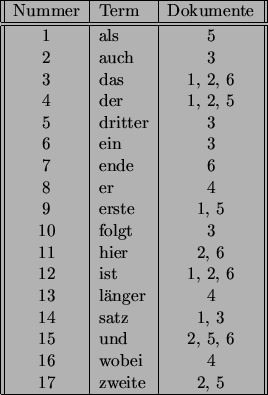
\includegraphics[scale=0.5]{../Abbildungen/index.png}
	\caption{Beispiel für einen invertierten Index \cite{index_Uni_Munich}}
\end{figure}

\subsection{Umsetzung eines invertierten Index}
Nachdem das Prinzip des invertierten Index klar ist, steht die Frage im Raum wie dieser umgesetzt werden kann.
Es liegt nahe als Datenstruktur einen Trie einzusetzen. Ein Trie ist ein spezieller Suchbaum, welcher besonders gut zum Suchen von Zeichenketten geeignet ist \cite{IR_Intro_Cambridge}.
\newline
Alternativ kann über den Einsatz einer Hasmap nachgedacht werden, jedoch führt dies zu folgendem Problem:
Angenommen eine vom Nutzer eingegebene Query ist nicht in der Hashmap vorhanden. Die Hash-Funktion wird einen Fehler werfen. Da in einer Hashmap Wörter, die ähnlich zueinander sind, nicht unbedingt benachbart gespeichert werden und keinerlei Information darüber bekannt ist, wo zur Query ähnliche Wörter gespeichert sind, kann im Falle, dass ein oder mehrere Wörter der Query nicht vorhanden sind, nicht mit geringem Aufwand nach ähnlichen Wörtern gesucht werden. Bei Tries besteht dieses Problem nicht \cite{IR_Intro_Cambridge}. 
\newline
Da in der Beispielimplementierung ein Trie als Datenstruktur zum Einsatz kommen wird, soll diese kurz vorgestellt werden.

\subsubsection{Tries}
Ein Trie wird auf der Basis einer Menge von Zeichenketten aufgebaut. Jede Zeichenkette, die gefunden werden muss, ist innerhalb des Tries repräsentiert.
\newline
Erreicht wird dies dadurch, dass ein Knoten jeweils ein Zeichen repräsentiert und eine Liste mit Verweisen auf die nächsten möglichen Knoten hält, basierend auf einem weiteren Zeichen.
Die folgende Abbildung zeigt einen Trie.

\begin{figure}[H]
	\centering
	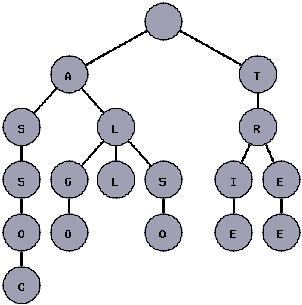
\includegraphics[scale=0.7]{../Abbildungen/trie.png}
	\caption{Beispiel eines Tries \cite{trie_Abb}}
\end{figure}

\newpage
Im Folgenden soll eine formale Definition eines Tries gegeben werden:
\newline
\begin{defi}
	Sei $\sum$ eine endliche Menge von Zeichen (Alphabet) und $\sum^{*}$ die Menge aller Wörter, die über $\sum$ gebildet werden können. Sei $S$ $\subseteq$ $\sum^{*}$. Dann ist $T = (V, E)$ ein Trie, wobei $V$ die Menge aller Knoten und $E$ die Menge aller Kanten ist. Darüber hinaus muss gelten:
	
	\begin{itemize}
		\item $\forall e \in E: e$ ist mit Zeichen aus $\sum$ beschriftet.
		\item $\forall v \in V:$ alle ausgehenden Kanten von $v$ sind unterschiedlich beschriftet mit einem Zeichen $z \in \sum$
		\item $\forall S_i \in S: \exists v \in V: S_i$ ist ein Präfix der Konkatenation der Beschriftungen des Pfades vom Wurzelknoten bis $v$.
		\item $\forall b \in V: \exists S_i \in S:$ Die Konkatenation der Beschriftungen von der Wurzel bis $b$ ergibt $S_i$, sofern $b$ ein Blatt des Tries ist.
	\end{itemize}
\end{defi}

Definition 2.7 ist aus \cite{Trie_wiki} entnommen.
\newline \newline
Das Suchen nach gespeicherten Wörtern gestaltet sich nun verhältnismäßig einfach: Um das Wort \glqq Tree\grqq im, in der Abbildung gezeigten, Trie zu finden, wird wie folgt vorgegangen.
\newline 
Stellt der User die Anfrage \glqq Tree\grqq wird diese Query nun Zeichen für Zeichen durchgegangen. Beginnend bei \glqq T\grqq wird im Wurzelknoten geprüft, ob es einen Verweis auf einen Knoten gibt, der ein \glqq T\grqq repräsentiert \cite{trie_Abb}. Existiert ein solcher Knoten, wird in diesem geprüft, ob es einen Knoten gibt, der das nächste Zeichen in der Query (das \glqq r\grqq) repräsentiert. Ist dies der Fall wird das Verfahren solange wiederholt bis die Query komplett eingelesen ist oder in der Query ein Zeichen steht, das durch keinen Knoten im Trie repräsentiert ist \cite{trie_Abb} \cite{Trie_Blog}.
\newline \newline
Ähnlich leicht funktioniert das Einfügen neuer Wörter in den Trie. Dazu wird - wie beim Suchen - das Wort, das eingefügt werden soll, so weit wie möglich nach dem oben beschriebenen Muster eingelesen und es wird zu den entsprechenden Knoten gesprungen \cite{trie_Abb} \cite{Trie_Blog}. Wird nun ein Zeichen eingelesen, das nicht durch einen Knoten repräsentiert ist, wird ein neuer Knoten erzeugt, welcher dieses Zeichen repräsentiert \cite{trie_Abb}. Alle nun noch einzulesenden Zeichen erhalten einen neuen Knoten, da der neu erzeugte Knoten natürlich nicht auf bereits vorhandene Knoten zeigen kann. Innerhalb dieses Knotens wird eine Liste angelegt, die Verweise auf weitere Knoten hält \cite{trie_Abb}. In dieser Liste wird ein Verweis auf den Knoten angelegt, der das nächste Zeichen des einzufügenden Wortes repräsentiert. Dieses Verfahren setzt sich solange fort, bis das neue Wort vollständig eingelesen ist.
\newline \newline
Das Löschen soll in diesem Rahmen nicht aufgezeigt werden, da dies weitaus komplexer sein kann als das Finden oder Einfügen von Einträgen.
\newline \newline
Ein Knoten, zu dem man mit dem Wort $S_i$ gelangt, muss außerdem eine Liste mit Verweisen auf alle Dokumente, in denen das Wort $S_i$ vorkommt, speichern. Gibt es keine Dokumente, in denen $S_i$ vorkommt, ist die Liste leer.

\section{Komprimierung des Index}
Bei großen Dokumentenmengen wächst die Größe des Index ebenfalls. Doch nicht nur die Größe des Index wächst, sondern auch die benötigte Zeit, um auf eine Query zu antworten \cite{IR_Intro_Cambridge}.
Die Index-Komprimierung adressiert genau dieses Problem. Über die Jahre der Forschung haben sich einige Komprimierungs-Techniken bewährt und sind bei den allermeisten aktuellen Suchmaschinen in Benutzung. \newline
Dieser Abschnitt soll das Thema Komprimierung erläutern, das Hauptaugenmerk liegt dabei auf der Komprimierungs-Technik, die in der Beispielimplementierung eingesetzt wird.

\subsection{Nutzen der Komprimierung}
Bevor die technischen Details der Komprimierung betrachtet werden, sollen zunächst die Vorteile, die sich durch die Komprimierung ergeben, aufgezeigt werden.
\\
In erster Linie wird durch die Komprimierung Platz auf dem Speichermedium, auf dem der Index liegt, gespart. Liegt dieser beispielsweise in einer Datei auf einer Festplatte, zieht die Komprimierung noch weitere Vorteile mit sich: Bei Schreib- bzw. Leseoperationen auf die Datei, müssen durch die Komprimierung weniger Bytes vom Hauptspeicher zur Festplatte bzw. umgekehrt, transportiert werden. Dadurch verringert sich die I/O-Zeit \cite[S. 58, 86]{IR_Intro_Cambridge}. Weiter kann ein größerer Teil des Indexes im Cache gehalten werden, was den Zugriff auf den Index beschleunigt, da weniger I/O-Operationen auf der Festplatte erforderlich sind \cite[S. 58, 86]{IR_Intro_Cambridge}.

\subsection{Dictionary komprimieren}
In \ref{txt:inverted_index} wurde beschrieben, dass sich der invertierte Index in das Dictionary und die Posting-Listen aufteilt.
Dies sind die beiden Punkte, an denen bei der Komprimierung angesetzt werden kann.
Die erste Möglichkeit, die genauer betrachtet werden soll, ist die Dictionary-Kompression.
Der Idee, die betrachtet werden soll, liegt zugrunde, dass in der Datenstruktur, die zur Suche der Wörter, die in der Query enthalten sind, genutzt wird, in jedem Knoten ein Zeichen gespeichert wird. Wird UTF-8 zur Zeichencodierung verwendet, fällt pro Zeichen mindestens $1$ Byte an, das in jedem Knoten gespeichert werden muss. Meist besteht ein in UTF-8 codiertes Zeichen jedoch aus mehr als einem Byte. \\
Eine Möglichkeit, Speicherplatz zu sparen, ist, nicht ein Zeichen pro Konten zu speichern, sondern lediglich einen Pointer auf ein Zeichen. Der Pointer wird als Index auf eine Liste verwendet, welche alle Zeichen enthält, die in den Dokumenten, die der Index \glqq kennt\grqq. Ist die dem Index zugrunde liegende Datenstruktur ein B-Baum oder ein Binärbaum, kann noch weiter Speicherplatz gespart werden, indem der Liste Teilstrings hinzugefügt werden, die in mehreren Wörtern vorkommen. Da im Rahmen dieser Arbeit jedoch ein Trie verwendet wird, wird dieser Punkt nicht weiter betrachtet, da ein Trie eine solche Komprimierung bereits liefert, da jeder Substring lediglich ein mal abgespeichert wird.
\\
\\
Ein Beispiel soll aufzeigen, wie mittels Pointern Speicherplatz gespart werden kann. Dazu zunächst eine Rechnung, wie viel Speicherplatz durch Zeichen in einem klassischen Trie benötigt wird:
Sei $T_1$ ein Trie mit einer Knotenzahl von $15$ Knoten. Jeder der Knoten beinhaltet ein Zeichen, welches jeweils $2$ Byte benötigt. Somit werden $15 \ * \ 2 \ = \ 30$ Byte benötigt, um alle Zeichen zu speichern. 
\\
Wird nun die Dictionary-Komprimierung angewendet, so wird eine Liste mit allen Zeichen, die in den eingelesenen Dokumenten vorkommen, angelegt. Die Größe dieser Liste bleibt beim Hinzufügen neuer Dokumente in den Index konstant, sofern die Dokumente keine bisher unbekannten Zeichen beinhalten. Die Größe der Liste ist somit für große Tries, wie sie in einem Index gewöhnlicherweise entstehen, vernachlässigbar. 
\\
Die Liste $l$ habe $26$ Einträge und beinhaltet das Alphabet von a-z ohne Umlaute.
Jeder Knoten im Trie muss jetzt lediglich einen Zeiger auf einen Listeneintrag abspeichern. Damit werden nur noch $log_2(26) \approx 4,7$ Bits benötigt. Da aufgerundet werden muss, werden 5 Bits zum Speichern des Zeigers benötigt. Damit wird eine Einsparung von $11$ Bits pro Knoten erreicht, wodurch im gesamten Trie $T_1$ $11 \ * \ 15  \ = \ 165$ Bits eingespart werden, was $20$ Bytes entspricht.
\\
Um noch weitere Zeichen in die Liste aufnehmen zu können, kann pro Zeiger ein Byte genutzt werden. Dadurch können $256$ Zeichen unterstützt werden und dennoch werden im Trie $T_1$ $15$ Bytes eingespart.
Dies wird Byte-Alignment genannt.
\\
In diesem Beispiel scheint sich der Nutzen der Komprimierung in Grenzen zu halten, betrachtet man jedoch einen Trie $T_2$ mit einer Knotenzahl von $10.000$, ergibt sich ein anderes Bild: 
Statt $10.000 \ * \ 2 = 20.000$ Byte werden mit Byte-Alignment nur noch $10.000$ Byte benötigt, wodurch $50\%$ Speicherplatz gespart werden, sofern der marginale Speicherbedarf der Liste $l$ nicht mit einbezogen wird.

\subsection{Postings-Liste komprimieren}
Weitaus mehr Speicher wird von den Posting-Listen benötigt, die im Index gespeichert werden müssen. Zur Erinnerung: Die Einträge in einer Posting-Liste verweisen auf diejenigen Dokumente, in denen das entsprechende Wort bzw. der entsprechende Term vorkommt.
\\
Der Speicherbedarf der Posting-Listen über den gesamten Index kann nicht so einfach berechnet werden, wie der Speicherbedarf des Dictionarys. Im Falle eines Tries lässt sich die Anzahl der benötigten Bytes für das Dictionary mit $ Anzahl \ Knoten \ * \ Bytes \ pro \ Zeichen$ berechnen. Da die Posting-Listen jedoch unterschiedliche Längen pro Knoten aufweisen, lässt sich keine solch einfach Formel finden.
\\
Durchschnittlich benötigen Posting-Listen mehr Speicher pro Knoten als die Byteanzahl eines zu speichernden Zeichens. Werden die Dokumenten-IDs (oder Postings) mit 4-Byte-Integern abgespeichert, benötigt eine Liste $l$ $|l| \ * \ 4$ Bytes. mit 4-Byte-Integern können auf $2^{32}$ Dokumente referenziert werden, was bei großen Dokumentenmengen schnell zu Problemen führt, da weit mehr Dokumente im Index aufgenommen werden müssen. Werden 8-Byte-Integer genutzt, so können $2^{64}$ Dokumente referenziert werden, die Posting-Liste $l$ benötigt dann $|l| \ * \ 8$ Byte.
\\
Werden in der Liste statt der echten Dokumenten-ID lediglich die Differenzen zwischen den einzelnen Einträgen gespeichert, können kleinere Zahlen genutzt werden. Die folgenden zwei Tabellen zeigen, wie das aussehen könnte:


\\
Kleinere Zahlen können mit weniger Bits codiert werden, wie dies umgesetzt wird, ist Gegenstand der nächsten Abschnitte.
Es gibt mehrere Verfahren, wie diese Liste komprimiert werden kann bzw. die Integer-Werte, die in der Liste enthalten sind. Es wird dabei zwischen byte- und bit-orientierten Codes unterschieden. Im Folgenden werden zwei Varianten vorgestellt, Variable Byte Encoding und $\gamma$-Codes.

\subsubsection{Variable Byte Encoding (VBE)}
Dieser Code fällt - wie der Name bereits zeigt - in die Kategorie der byte-orientierten Komprimierung.
\\
In den meisten Computersystemen werden Integer als 4-Byte-Integer dargestellt.
Wie oben gezeigt, müssen jedoch nur noch kleine Zahlen gespeichert werden. Es wäre Verschwendung, kleine Zahlen, die mithilfe ein oder zwei Bytes codiert werden können, als 4-Byte-Integer abzuspeichern, bei dem zwei Byte lediglich führende 0en darstellen.
\\



\section{TF-IDF Gewichtung}


\section{Retrieval}
%---------------------------------------------------------------------------------	
		\chapter{Invertierter Index}
		\label{invertindex}
		Dieser Abschnitt wird die Idee des invertierten Index vorstellen sowie die Erzeugung des invertierten Index erläutern. Darüber hinaus wird aufgezeigt, wie die Verarbeitung einer Query mittels des invertierten Index funktioniert. Ab jetzt werden die Ausdrücke \glqq invertierter Index\grqq\ und \glqq Index\grqq\ synonym verwendet.
\section{Grundlegender Aufbau}
Der invertierte Index kann als ein Dictionary betrachtet werden, welches für jeden Term, der in der Dokumentenmenge vorkommt, einen Eintrag hält \cite{IR_Intro_Cambridge} \cite{IR_Uni_Bamberg}. Dieser Eintrag wiederum ist eine Liste. Diese hält mindestens eine eindeutige Dokumenten-ID, meist jedoch darüber hinaus weitere Informationen. Beispiele für solche weiteren Informationen sind Häufigkeit, in der ein Term in einem Dokument vorkommt, die Position und die umliegenden Wörter in der Nähe zum Term $t$ \cite{IR_Intro_Cambridge}.
Die Listen, die zu jedem Term angelegt werden, heißen Posting-Listen \cite{IR_Intro_Cambridge}.
\newline
Den invertierten Index kann man folgendermaßen visualisieren:
\begin{figure}[H]
	\centering
	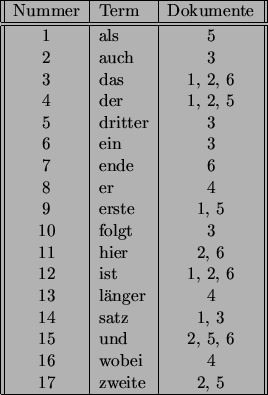
\includegraphics[scale=0.5]{../Abbildungen/index.png}
	\caption{Beispiel für einen invertierten Index \cite{index_Uni_Munich}}
\end{figure}

\section{Umsetzung eines invertierten Index}
Nachdem das Prinzip des invertierten Index klar ist, steht die Frage im Raum wie dieser umgesetzt werden kann.
Es liegt nahe als Datenstruktur einen Trie einzusetzen. Ein Trie ist ein spezieller Suchbaum, welcher besonders gut zum Suchen von Zeichenketten geeignet ist \cite{IR_Intro_Cambridge}.
\newline
Alternativ kann über den Einsatz einer Hashmap nachgedacht werden, jedoch führt dies zu folgendem Problem:
Angenommen die Terme einer vom Nutzer eingegebenen Query sind nicht in der Hashmap vorhanden, dann wird die Hash-Funktion keinen passenden Eintrag finden. Da in einer Hashmap Wörter, die ähnlich zueinander sind, nicht unbedingt benachbart gespeichert werden und keinerlei Information darüber bekannt ist, wo zur Query ähnliche Wörter gespeichert sind, kann im Falle, dass ein oder mehrere Wörter der Query nicht vorhanden sind, nicht mit geringem Aufwand nach ähnlichen Wörtern gesucht werden. Bei Tries besteht dieses Problem nicht \cite{IR_Intro_Cambridge}. 
\newline
\begin{comment}
	Da in der Beispielimplementierung ein Trie als Datenstruktur zum Einsatz kommen wird, soll diese kurz vorgestellt werden.
\end{comment}

Da die Beispiel-Implementierung, die später vorgestellt wird, jedoch möglichst einfach sein soll, wird zunächst eine Hashmap als Datenstruktur verwendet. 

\subsection{Tries}
Ein Trie wird auf der Basis einer Menge von Zeichenketten aufgebaut. Jede Zeichenkette, die gefunden werden muss, ist innerhalb des Tries repräsentiert.
\newline
Erreicht wird dies dadurch, dass ein Knoten jeweils ein Zeichen repräsentiert und eine Liste mit Verweisen auf die nächsten möglichen Knoten hält, basierend auf einem weiteren Zeichen.
Die folgende Abbildung zeigt einen Trie.

\begin{figure}[H]
	\centering
	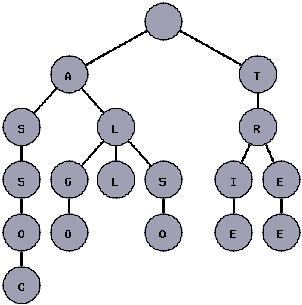
\includegraphics[scale=0.7]{../Abbildungen/trie.png}
	\caption{Beispiel eines Tries \cite{trie_Abb}}
\end{figure}

\newpage
Im Folgenden soll eine formale Definition eines Tries gegeben werden:
\newline
\begin{defi}
	Sei $\sum$ eine endliche Menge von Zeichen (Alphabet) und $\sum^{*}$ die Menge aller Wörter, die über $\sum$ gebildet werden können. Sei $S$ $\subseteq$ $\sum^{*}$. Dann ist $T = (V, E)$ ein Trie, wobei $V$ die Menge aller Knoten und $E$ die Menge aller Kanten ist. Darüber hinaus muss gelten:
	
	\begin{itemize}
		\item $\forall e \in E: e$ ist mit Zeichen aus $\sum$ beschriftet.
		\item $\forall v \in V:$ alle ausgehenden Kanten von $v$ sind unterschiedlich beschriftet mit einem Zeichen $z \in \sum$
		\item $\forall S_i \in S: \exists v \in V: S_i$ ist ein Präfix der Konkatenation der Beschriftungen des Pfades vom Wurzelknoten bis $v$.
		\item $\forall b \in V: \exists S_i \in S:$ Die Konkatenation der Beschriftungen von der Wurzel bis $b$ ergibt $S_i$, sofern $b$ ein Blatt des Tries ist.
	\end{itemize}
\end{defi}

Definition 2.7 ist aus \cite{Trie_wiki} entnommen.
\newline \newline
Das Suchen nach gespeicherten Wörtern gestaltet sich nun verhältnismäßig einfach: Um das Wort \glqq Tree\grqq\ im, in der Abbildung gezeigten, Trie zu finden, wird wie folgt vorgegangen:
\newline 
Stellt der User die Anfrage \glqq Tree\grqq, wird diese Query nun Zeichen für Zeichen durchgegangen. Beginnend bei \glqq T\grqq\ wird im Wurzelknoten geprüft, ob es einen Verweis auf einen Knoten gibt, der ein \glqq T\grqq\ repräsentiert \cite{trie_Abb}. Existiert ein solcher Knoten, wird in diesem geprüft, ob es einen Knoten gibt, der das nächste Zeichen in der Query (das \glqq r\grqq) repräsentiert. Ist dies der Fall, wird das Verfahren solange wiederholt, bis die Query komplett eingelesen ist oder in der Query ein Zeichen steht, das durch keinen Knoten im Trie repräsentiert ist \cite{trie_Abb} \cite{Trie_Blog}.
\newline \newline
Ähnlich leicht funktioniert das Einfügen neuer Wörter in den Trie. Dazu wird - wie beim Suchen - das Wort, das eingefügt werden soll, so weit wie möglich nach dem oben beschriebenen Muster eingelesen und es wird zu den entsprechenden Knoten gesprungen \cite{trie_Abb} \cite{Trie_Blog}. Wird nun ein Zeichen eingelesen, das nicht durch einen Knoten repräsentiert ist, wird ein neuer Knoten erzeugt, welcher dieses Zeichen repräsentiert \cite{trie_Abb}. Alle nun noch einzulesenden Zeichen erhalten einen neuen Knoten, da der neu erzeugte Knoten natürlich nicht auf bereits vorhandene Knoten zeigen kann. Innerhalb dieses Knotens wird eine Liste angelegt, die Verweise auf weitere Knoten hält \cite{trie_Abb}. In dieser Liste wird ein Verweis auf den Knoten angelegt, der das nächste Zeichen des einzufügenden Wortes repräsentiert. Dieses Verfahren setzt sich solange fort, bis das neue Wort vollständig eingelesen ist.
\newline \newline
Das Löschen soll in diesem Rahmen nicht aufgezeigt werden, da dies weitaus komplexer sein kann als das Finden oder Einfügen von Einträgen.
\newline \newline
Ein Knoten, zu dem man mit dem Wort $S_i$ gelangt, muss außerdem eine Liste mit Verweisen auf alle Dokumente, in denen das Wort $S_i$ vorkommt, speichern. Gibt es keine Dokumente, in denen $S_i$ vorkommt, ist die Liste leer.

\begin{comment}
\section{Komprimierung des Index}
Bei großen Dokumentenmengen wächst die Größe des Index ebenfalls. Doch nicht nur die Größe des Index wächst, sondern auch die benötigte Zeit, um auf eine Query zu antworten \cite{IR_Intro_Cambridge}.
Die Index-Komprimierung adressiert genau dieses Problem. Über die Jahre der Forschung haben sich einige Komprimierungs-Techniken bewährt und sind bei den allermeisten aktuellen Suchmaschinen in Benutzung. \newline
Dieser Abschnitt soll das Thema Komprimierung erläutern, das Hauptaugenmerk liegt dabei auf der Komprimierungs-Technik, die in der Beispielimplementierung eingesetzt wird.

\subsection{Nutzen der Komprimierung}
Bevor die technischen Details der Komprimierung betrachtet werden, sollen zunächst die Vorteile, die sich durch die Komprimierung ergeben, aufgezeigt werden.
\\
In erster Linie wird durch die Komprimierung Platz auf dem Speichermedium, auf dem der Index liegt, gespart. Liegt dieser beispielsweise in einer Datei auf einer Festplatte, zieht die Komprimierung noch weitere Vorteile mit sich: Bei Schreib- bzw. Leseoperationen auf die Datei, müssen durch die Komprimierung weniger Bytes vom Hauptspeicher zur Festplatte bzw. umgekehrt, transportiert werden. Dadurch verringert sich die I/O-Zeit \cite[S. 58, 86]{IR_Intro_Cambridge}. Weiter kann ein größerer Teil des Indexes im Cache gehalten werden, was den Zugriff auf den Index beschleunigt, da weniger I/O-Operationen auf der Festplatte erforderlich sind \cite[S. 58, 86]{IR_Intro_Cambridge}.

\subsection{Dictionary komprimieren}
In \ref{txt:inverted_index} wurde beschrieben, dass sich der invertierte Index in das Dictionary und die Posting-Listen aufteilt.
Dies sind die beiden Punkte, an denen bei der Komprimierung angesetzt werden kann.
Die erste Möglichkeit, die genauer betrachtet werden soll, ist die Dictionary-Kompression.
Der Idee, die betrachtet werden soll, liegt zugrunde, dass in der Datenstruktur, die zur Suche der Wörter, die in der Query enthalten sind, genutzt wird, in jedem Knoten ein Zeichen gespeichert wird. Wird UTF-8 zur Zeichencodierung verwendet, fällt pro Zeichen mindestens $1$ Byte an, das in jedem Knoten gespeichert werden muss. Meist besteht ein in UTF-8 codiertes Zeichen jedoch aus mehr als einem Byte. \\
Eine Möglichkeit, Speicherplatz zu sparen, ist, nicht ein Zeichen pro Knoten zu speichern, sondern lediglich einen Pointer auf ein Zeichen. Der Pointer wird als Index auf eine Liste verwendet, welche alle Zeichen enthält, die in den Dokumenten vorkommen, die der Index \glqq kennt\grqq. Ist die dem Index zugrunde liegende Datenstruktur ein B-Baum oder ein Binärbaum, kann noch weiter Speicherplatz gespart werden, indem der Liste Teilstrings hinzugefügt werden, die in mehreren Wörtern vorkommen. Da im Rahmen dieser Arbeit jedoch ein Trie verwendet wird, wird dieser Punkt nicht weiter betrachtet, da ein Trie eine solche Komprimierung bereits liefert, da jeder Substring lediglich einmal abgespeichert wird.
\\
\\
Ein Beispiel soll aufzeigen, wie mittels Pointern Speicherplatz gespart werden kann. Dazu zunächst eine Rechnung, wie viel Speicherplatz durch Zeichen in einem klassischen Trie benötigt wird:
Sei $T_1$ ein Trie mit einer Knotenzahl von $15$ Knoten. Jeder der Knoten beinhaltet ein Zeichen, welches jeweils $2$ Byte benötigt. Somit werden $15 \ * \ 2 \ = \ 30$ Byte benötigt, um alle Zeichen zu speichern. 
\\
Wird nun die Dictionary-Komprimierung angewendet, so wird eine Liste mit allen Zeichen, die in den eingelesenen Dokumenten vorkommen, angelegt. Die Größe dieser Liste bleibt beim Hinzufügen neuer Dokumente in den Index konstant, sofern die Dokumente keine bisher unbekannten Zeichen beinhalten. Die Größe der Liste ist somit für große Tries, wie sie in einem Index gewöhnlicherweise entstehen, vernachlässigbar. 
\\
Die Liste $l$ habe $26$ Einträge und beinhaltet das Alphabet von a-z ohne Umlaute.
Jeder Knoten im Trie muss jetzt lediglich einen Zeiger auf einen Listeneintrag abspeichern. Damit werden nur noch $log_2(26) \approx 4,7$ Bits benötigt. Da aufgerundet werden muss, werden 5 Bits zum Speichern des Zeigers benötigt. Damit wird eine Einsparung von $11$ Bits pro Knoten erreicht, wodurch im gesamten Trie $T_1$ $11 \ * \ 15  \ = \ 165$ Bits eingespart werden, was $20$ Bytes entspricht.
\\
Um noch weitere Zeichen in die Liste aufnehmen zu können, kann pro Zeiger ein Byte genutzt werden. Dadurch können $256$ Zeichen unterstützt werden und dennoch werden im Trie $T_1$ $15$ Bytes eingespart.
Dies wird Byte-Alignment genannt.
\\
In diesem Beispiel scheint sich der Nutzen der Komprimierung in Grenzen zu halten, betrachtet man jedoch einen Trie $T_2$ mit einer Knotenzahl von $10.000$, ergibt sich ein anderes Bild: 
Statt $10.000 \ * \ 2 = 20.000$ Byte werden mit Byte-Alignment nur noch $10.000$ Byte benötigt, wodurch $50\%$ Speicherplatz gespart werden, sofern der marginale Speicherbedarf der Liste $l$ nicht mit einbezogen wird.

\subsection{Postings-Liste komprimieren}
Weitaus mehr Speicher wird von den Posting-Listen benötigt, die im Index gespeichert werden müssen. Zur Erinnerung: Die Einträge in einer Posting-Liste verweisen auf diejenigen Dokumente, in denen das entsprechende Wort bzw. der entsprechende Term vorkommt.
\\
Der Speicherbedarf der Posting-Listen über den gesamten Index kann nicht so einfach berechnet werden wie der Speicherbedarf des Dictionarys. Im Falle eines Tries lässt sich die Anzahl der benötigten Bytes für das Dictionary mit $ Anzahl \ Knoten \ * \ Bytes \ pro \ Zeichen$ berechnen. Da die Posting-Listen jedoch unterschiedliche Längen pro Knoten aufweisen, lässt sich keine solch einfache Formel finden.
\\
Durchschnittlich benötigen Posting-Listen mehr Speicher pro Knoten als die Byteanzahl eines zu speichernden Zeichens. Werden die Dokumenten-IDs (oder Postings) mit 4-Byte-Integern abgespeichert, benötigt eine Liste $l$ $|l| \ * \ 4$ Bytes. mit 4-Byte-Integern können auf $2^{32}$ Dokumente referenziert werden, was bei großen Dokumentenmengen schnell zu Problemen führt, da weit mehr Dokumente im Index aufgenommen werden müssen. Werden 8-Byte-Integer genutzt, so können $2^{64}$ Dokumente referenziert werden, die Posting-Liste $l$ benötigt dann $|l| \ * \ 8$ Byte.
\\
Werden in der Liste statt der echten Dokumenten-ID lediglich die Differenzen zwischen den einzelnen Einträgen gespeichert, können kleinere Zahlen genutzt werden. Die folgenden zwei Tabellen zeigen, wie das aussehen könnte:


\\
Kleinere Zahlen können mit weniger Bits codiert werden, wie dies umgesetzt wird, ist Gegenstand der nächsten Abschnitte.
Es gibt mehrere Verfahren, wie diese Liste komprimiert werden kann bzw. die Integer-Werte, die in der Liste enthalten sind. Es wird dabei zwischen byte- und bit-orientierten Codes unterschieden. Im Folgenden werden zwei Varianten vorgestellt, Variable Byte Encoding und $\gamma$-Codes.

\subsubsection{Variable Byte Encoding (VBE)}
Dieser Code fällt - wie der Name bereits zeigt - in die Kategorie der byte-orientierten Komprimierung.
\\
In den meisten Computersystemen werden Integer als 4-Byte-Integer dargestellt.
Wie oben gezeigt, müssen jedoch nur noch kleine Zahlen gespeichert werden. Es wäre Verschwendung, kleine Zahlen, die mithilfe ein oder zwei Bytes codiert werden können, als 4-Byte-Integer abzuspeichern, bei dem zwei Byte lediglich führende 0en darstellen.
\\
\end{comment}
%---------------------------------------------------------------------------------
		\chapter{TF-IDF}
		\label{tfidf}
		Bei großen Sammlungen von Dokumenten reicht es nicht aus, wenn das IR die Dokumente zurückgibt, welche die Suchanfrage erfüllen. Die Menge der Dokumente, die durch das IR zurückgegebene werden, ist meist zu groß, so dass der Nutzer nicht in der Lage ist alle Dokumente zu sichten und die für ihn relevanten Dokument auszuwählen.\\
Die Frage, die sich hier stellt, ist, wie der Nutzer die Dokumente bekommt, die er mit hoher wahrscheinlichsten benötigt. Hier fällt der Begriff des Scorings. Scoring oder auch Bewertung wird genutzt um zu bestimmen, welche Dokumente für die Suchanfrage am relevantesten sind. Es kann auch von einer Gewichtung der Dokumente gesprochen werden.\\
Das Gewichtungsmodell, welches in dieser Arbeit thematisiert und genutzt wird, ist das TF-IDF-Maß. Da es sich bei der Eingabe des Nutzers um Freitext handelt und nicht um Terme, welche durch logische Operatoren verknüpft werden, bietet sich das TF-IDF-Maß an. TF steht hierbei für Term Frequency und IDF für Inverse Document Frequency. Beide Methoden werde einzeln in den folgenden Abschnitten vorgestellt und am Ende verknüpft.

\section{Term Frequency}
Um Dokumente aus einer Kollektion nach Termen einer Suchquery zu gewichten, ist das zählen der Terme $t$ einer Query in jedem Dokument $d$ die zunächst trivialste Lösung. Denn ein Dokument welches einen Term öfter besitzt, als ein anderes Dokument, hat mehr mit der Suchquery zu tun und muss dementsprechend höher gewichtet werden. Bei dieser Vorgehensweise wird von Term Frequency (siehe \cref{def:TF}) gesprochen, auf deutsch auch als Suchwortdichte bekannt. \newpage
\begin{defi}[Term Frequency]\label{def:TF}
	Die Term Frequency $tf_d,_t$ gibt die Anzahl des Terms $t$ in dem Dokument $d$ wider.
\end{defi}
Bei dieser Vorgehensweise werden jedoch nicht die Anordnung der Terme sowohl im Dokument, als auch in der Query berücksichtigt. Die Query \glqq Karl ist engagierter als Eckhard\grqq\ liefert die gleiche Gewichtung für die Dokumente einer Kollektion zurück wie \glqq Eckhard ist engagierter als Karl\grqq . Dieses Modell, das die Anordnung der Terme innerhalb des Dokumentes ignoriert, wird auch als \glqq Bag of Words Model\grqq\ bezeichnet und beschreibt, dass ein Dokument, eine Menge von Wörter und deren Anzahl ist. Das bedeutet, dass zwei Dokumente, welche die selben Wörter und die selbe Anzahl dieser haben, als identisch angesehen werden, obwohl sie das nicht unbedingt sind. Des Weiteren werden alle Terme als gleich wichtig gewertet, welches nicht immer zielführend ist, wie in Abschnitt \ref{sub:tokenerzeugung} mit den \glqq stop words\grqq\ beschrieben wurde.

\section{Inverse Document Frequency}
Da die Terme in einer Suchquery nicht alle von gleicher Bedeutung für die Suche sind, muss eine Lösung gefunden werden, wie die Terme untereinander gewichtet. Hier fällt der Begriff der Document Frequency (siehe \cref{def:DF})

\begin{defi}[Document Frequency]\label{def:DF}
	Die Document Frequency $df_t$ gibt die Anzahl der Dokumente $d$ in der genutzten Kollektion an, welche den Term $t$ besitzen.
\end{defi}

\begin{defi}[Inverse Document Frequency]\label{def:IDF}
	$IDF_t = log(\frac{N_D}{df_t})$
\end{defi}

Durch die Document Frequency kann festgestellt werden,

\section{Das TF-IDF-Maß}

\begin{defi}[TF-IDF]\label{defi:TF-IDF}
	Inhalt...
\end{defi}
%---------------------------------------------------------------------------------
		\chapter{Implementierung - Lokale Suchmaschine}
		\label{impl}
		\section{Ziel der Beispiel-Implementierung}\label{ziel-der-beispiel-implementierung}

Im Folgenden wird eine Beispiel-Implementierung der zuvor theoretisch diskutierten Inhalte vorgestellt. Dabei wird eine lokale Suchmaschine entwickelt, welche in der Lage ist, PDF-Dateien auf einem lokalen Computer-System zu parsen, in einen invertierten Index aufzunehmen, sowie Suchanfragen eines Benutzers sinnvoll zu beantworten. Zur Relevanz-Bestimmung der Dokumente wird das TF-IDF-Maß, welches bereits vorgestellt wurde, genutzt. Das Speichern des Index wird mit der von Python mitgelieferte Datenstruktur \textit{Dictionary}, welche im Grunde eine Hashmap ist, umgesetzt. Weiter werden Bibliotheken eingesetzt, welche einige Vorarbeit leisten und damit den Code der Beispiel-Implementierung auf das Wesentliche beschränken. Die Anwendung soll die grundlegende Arbeitsweise eines Information Retrieval-Systems darlegen.

\section{Genutzte Bibliotheken}\label{genutzte-bibliotheken}

Vor der eigentlichen Implementierung der lokalen Suchmaschine werden einige Module eingebunden (siehe Abbildung \ref{fig:import}), welche die Implementierung unterstützen. Im Folgenden werden die Module aufgelistet und wichtige Module im jeweiligen Abschnitt genauer erläutert:\newpage
\begin{itemize}
	\item Apache Tika: Erkennt und extrahiert Metadaten und Texte aus über tausend Dateitypen \cite{Apache_Tika}
	\item Math: Standard Python-Modul für mathematische Funktionen
	\item OS: Stellt Betriebssystem-Funktionalitäten bereit. Wird hier genutzt, um durch Verzeichnisse zu navigieren
	\item Filetype: Wird zur Dateityp-Erkennung genutzt \cite{filetype}
	\item RE: Das re-Modul stellt Funktionen bereit, mit denen mit regulären Ausdrücken gearbeitet werden kann. In der Beispiel-Implementierung werden mit diesem Modul die Tokens ermittelt. \cite{python_re}
	\item Platform: Prüfung, auf welchem Betriebssystem das Programm läuft, da Windows- und Linux-Systeme verschiedene Dateisysteme nutzen
	\item Operator: Dieses Modul exportiert effiziente Funktionen, die den eigentlichen Operatoren von Python entsprechen. Es findet nur Anwendung in der Sortierung der zu zurückgebenden Dokumente in der retrieve-Methode.
	\item NLTK: Stellt Funktionen zur Verfügung, die es ermöglichen mit menschlichen Sprachdaten zu arbeiten.
\end{itemize}

Die Module Apache Tika, Filetype sowie NLTK müssen per pip installiert werden und sind damit nicht standardmäßig in Python integriert.


\subsection{Apache Tika}\label{apache-tika}
Bei Apache Tika handelt es sich um eine Bibliothek, um Inhalte aus Dateien zu erkennen und zu analysieren. Es ist in der Lage Text und Metadaten aus verschiedenen Arten von Dateien zu extrahieren. Apache Tika liefert einen Parser, mit dessen Hilfe der Text aus - unter anderem - PDF-Dateien extrahiert werden kann. Mit dem Aufruf \textit{parser.from\_file(file)} kann ein PDF-Dokument in Text umgewandelt werden.

\subsection{filetype}\label{python-magic}
Mittels filetype ist es möglich, unabhängig von der Dateiendung, den Typ einer Datei zu ermitteln. Dies hat den Vorteil, dass die Suchmaschine sowohl unter Windows, als auch unter Unix-Systemen, alle PDF-Dateien finden kann, da unter Unix die Dateiendung keine garantierten Rückschlüsse auf den Typ der Datei zulässt.

\subsection{NLTK}\label{nltk}
NLTK (natural language toolkit) ist eine Bibliothek für Python, die für die Verarbeitung natürlicher Sprachen eingesetzt wird. Dabei bietet die Bibliotheken Funktionen für unter anderem Textklassifikation, Tokenisierung und Stemming.
In diesem Beispiel wird NLTK verwendet, um die Eingabetexte der Dokumente und die Eingaben des Nutzers zu Tokens zu verarbeiten. Dazu wird eine Klasse verwendet, die auf Basis von Regular Expressions arbeitet. Mehr dazu wird anhand der Implementierung gezeigt. %Zudem wird Stemming mithilfe von nltk durchgeführt, um Wörter auf ihren Wortstamm zurückzuführen. In den unteren Methoden wird näheres über die genutzten Operationen erläutert.

\subsection{Platform}
Das Platform-Modul wird in dieser Implementierung dazu verwendet, festzustellen, auf welchem Betriebssystem die lokale Suchmaschine ausgeführt wird. Dies muss ermittelt werden, da auf Windows und Linux unterschiedliche Dateisysteme arbeiten. In Linux ist das Startverzeichnis immer das Root-Verzeichnis (\glqq /\grqq). Unter Windows gibt meist mehrere Partitionen, die alle durchsucht werden müssen.

\begin{figure}
	\rule{\textwidth}{0.4pt}
		\begin{lstlisting}[language=Python]
from tika import parser
import filetype
import math
import os
import string
import platform
import operator
import re
from nltk.tokenize import RegexpTokenizer
		\end{lstlisting}
	\rule{\textwidth}{0.4pt}
	\caption{Imports}
	\label{fig:import}
\end{figure}

\section{Die Document-Klasse}\label{die-document-klasse}

Das Speichern der für das Retrieval wichtigen Informationen, geschieht mittels einer Document-Klasse (siehe Abbildung \ref{fig:document}). Diese Klasse hält unter anderem alle Member-Variablen, die wichtig sind, um das TF-IDF-Maß berechnen zu können. Die Member-Variablen der Klasse sind:
\begin{itemize}
	\item \textit{url}: String mit dem Pfad zum Dokument, welches von dieser Instanz repräsentiert wird
	\item \textit{length}: Integer, welcher die Anzahl der Wörter in diesem Dokument darstellt
	\item \textit{docId}: Integer, welcher dem Dokument einen eindeutigen Identifikator gibt
	\item \textit{score}: Float, welcher die Gewichtung der Dokument-Instanz zu einer Anfrage angibt
	\item \textit{termList}: Eine Liste von Strings, die die Terme des Dokumentes entsprechen. Diese wird durch die Methode \textit{\_preprocess} erzeugt (siehe Abschnitt \ref{preprocess})
\end{itemize} 

\begin{figure}
	\rule{\textwidth}{0.4pt}
		\begin{lstlisting}[language=Python]
class Document:

  def __init__(self, url, length, docId, termList):
    self.url = url
    self.length = length
    self.docId = docId
    self.score = 0.
    self.termList = termList
		\end{lstlisting}
	\rule{\textwidth}{0.4pt}
	\caption{Dokumentenklasse}
	\label{fig:document}
\end{figure}

Die Member-Variable \textit{url} soll am Ende des Retrievalprozesses zurückgegeben werden, da der Nutzer durch den Pfad direkten Zugriff auf das Dokument bekommt. Die Member-Variablen \textit{length}, \textit{termList} und \textit{score} werden für die Berechnung des TF-IDF-Maßes benötigt und so auch für den Retrievalprozess. Die Member-Variable \textit{docId} wird in der Indexklasse einerseits genutzt, um die Identifier in dem \textit{invIndex}-Dictionary den jeweiligen Termen zuzuordnen. Des Weiteren erfolgt die Zuordnung der jeweiligen ID zu ihrer Document-Instanz über die \textit{docHashmap} in der Indexklasse (siehe invIndex und docHashmap in Abschnitt \ref{der-index}).

\subsection{TF-IDF}\label{tf-idf}

Die Document-Klasse hält neben den benötigten Attributen auch die Scoringmethode \textit{tf\_idf} (siehe Abbildung \ref{fig:tfidf}). Dies ist die Implementierung des TF-IDF-Maßes und berechnet für jedes Dokument die Gewichtung für eine gegebene Suchquery. Hierbei benötigt die Funktion die Terme der Suchquery, welche über das Attribut \textit{queryTerms} übergeben werden. Das Attribut \textit{df} steht für die Document Frequency, welches für jeden Term die Anzahl der gefunden Dokumente in Form eines Dictionaries beinhaltet. Über das Attribut \textit{fileCount} wird die Anzahl der Dokumente in der Kollektion, hier die Dateien die im invertierten Index aufgenommen wurden, übergeben.

\begin{figure}
	\rule{\textwidth}{0.4pt}
		\begin{lstlisting}[language=Python]
def tf_idf(self, queryTerms, df, fileCount):

  tfDict = {}
  for term in queryTerms:
    tfDict[term] = 0  
  
  for term in self.termList:
    if term in queryTerms:
      tfDict[term] += 1

  for key, value in df.items():
    idf = math.log(fileCount/value+1)
    tfDict[key] *= idf

  self.score = sum(tfDict.values())

Document.tf_idf = tf_idf
		\end{lstlisting}
	\rule{\textwidth}{0.4pt}
	\caption{TF-IDF-Methode}
	\label{fig:tfidf}
\end{figure}

Als erstes wird das Dictionary \textit{tfDict} für die Term Frequency erstellt und mit den Termen der Query als Schlüssel und den Werten 0 initialisiert. In der nächsten For-Schleife wird über \textit{self.termList} iteriert, welches die Liste der Terme des Dokumentes ist. Wenn ein Term auch in der Suchquery enthalten ist, also \textit{term in queryTerms} zu true evaluiert wird, wird im \textit{tfDict} der Wert des gefunden Terms um eins aufaddiert. Am Ende enthält das \textit{tfDict} die Terme der Suchquery als Schlüssel und die Anzahl ihrer Vorkommnisse im Dokument als Wert, also die Term Frequency. Als letztes muss jede Term Frequency mit der Inverse Document Frequency multipliziert werden. Dafür wird über das Dictionary \textit{df} iteriert und für jedes Key-Value-Paar die Inverse Document Frequency ausgerechnet und auf die jeweilige Term Frequency multipliziert. Am Ende wird die Summe aller TF-IDF-Maße der \textit{score}-Variable zugeordnet und bilden so die finale Gewichtung für die gegebene Suche.

\section{Der Index}\label{der-index}

Die Index-Klasse beinhaltet alle Methoden um den invertierten Index aufzubauen und die \textit{retrieve}-Methode, welche die Dokumente, sortiert nach deren Gewicht, zu einer gegebenen Query zurückgibt (siehe Abbildung \ref{fig:index}). Folgenden Member-Variablen werden für den invertierten Indexaufbau und die \textit{retrieve}-Methode benötigt:

\begin{itemize}
	\item \textit{invIndex}: Ist ein Dictionary mit einem Term als Schlüssel und einer Menge von Dokumenten-IDs als Wert
	\item \textit{fileCount}: Zählt beim Aufbau des invertierten Indexes die Dokumente, die in diesem aufgenommen wurden
	\item \textit{docHashmap}: Ist ein Dictionary welches eine Dokumenten-ID ihrer zugehörige Document-Klasseninstanz zuordnet
\end{itemize}

Die Member-Variable \textit{invIndex} ist der invertierte Index welcher bei der \textit{retrieve}-Methode die Dokumenten-IDs zu einen gegebenen Term aus der Suchquery zurückgibt. Des Weiteren wird die Member-Variable \textit{docHashmap} dafür genutzt, um über die Dokumenten-IDs auf die jeweiligen Dokumentinstanzen zuzugreifen und so auf ihren Inhalt und die Scoringfunktion \textit{tf\_idf}. Die Member-Variable \textit{fileCount} gibt die Größe der Kollektion wieder und wird bei der Berechnung des TF-IDF-Maßes benötigt.

\begin{figure}
	\rule{\textwidth}{0.4pt}
		\begin{lstlisting}[language=Python]
class Index:
  
  def __init__(self):
    self.invIndex = {}
    self.fileCount = 0
    self.docHashmap = {}
		\end{lstlisting}
	\rule{\textwidth}{0.4pt}
	\caption{Indexklasse}
	\label{fig:index}
\end{figure}

\subsection{buildIndex}\label{buildindex}

Die Methode \emph{buildIndex} baut den invertierten Index auf und nutzt dafür die\\
\textit{\_getStartDirectories}- und die \textit{\_addToIndex}-Methode. Dabei kann der \textit{buildIndex}-Methode optional Startverzeichnisse in Form einer Liste mit raw Strings mitgegeben werden. In der ersten If-Abfrage wird geprüft, ob die Liste \textit{startDirectories} leer ist. Dies ist der Fall, wenn der Nutzer keine Startverzeichnisse mitgegeben hat. Dann werden die Startverzeichnisse mithilfe der \textit{\_getStartDirectories}-Methode ermittelt.

Der erste Schritt stellt das Iterieren über alle Startverzeichnisse der Liste \textit{startDirectories} dar. Anschließend werden für das Startverzeichnis, und alle darunterliegenden Verzeichnisse, bis zur untersten Ebene, die Dateien mithilfe der \textit{os.walk}-Funktion geholt. Für jede Datei wird dann mit den Funktionen \textit{os.path.abspath} und \textit{os.path.join} der absolute Pfad gebildet. Danach wird durch das Modul \textit{filetype} ermittelt, ob es sich um ein PDF-Dokument handelt. Ist ein Dokument vom Typ PDF, wird mithilfe des \textit{Tika}-Moduls, genauer gesagt mit dem \textit{parser}-Objekt, der Text aus dem PDF-Dokument extrahiert. Dies geschieht in dem die Methode \textit{from\_file} des Parsers, mit dem Pfad der Datei als Argument, aufgerufen wird. Bei der Rückgabe kann mithilfe des Schlüssels \textit{content} auf den Text zugegriffen werden, welcher dann in der Variable \textit{rawText} gespeichert wird.

Für jede entdeckte PDF-Datei wird die Member-Variable \textit{fileCount} um eins erhöht. Da die Zahl sich bei jedem gefunden Dokument ändert, wird diese gleich als Dokumenten-ID genutzt, da sie für jedes Dokument eindeutig ist. Im Folgenden Schritt wird der \textit{rawText} mithilfe der \textit{\_preprocessText}-Methode normalisiert, in eine Liste von Tokens geteilt und in der Liste \textit{processedText} gespeichert. Nun sind alle Daten vorhanden um eine Documentinstanz zu erstellen. Diese enthält, wie in Abschnitt \ref{die-document-klasse} schon beschrieben, den Pfad zum Dokument, die Anzahl der Wörter, die Dokumenten-ID und den Text als Liste von Tokens.

Im vorletztem Schritt wird die erstellte Document-Instanz seiner Dokumenten-ID in der Member-Variable \textit{docHashmap} zugeordnet, um später auf diese Instanz zurückgreifen zu können. Als letztes wird der invertierte Index, mithilfe der \textit{\_addToIndex}-Methode, der Tokenliste \textit{processedText} und der Dokumenten-ID, aktualisiert.

\begin{figure}
	\rule{\textwidth}{0.4pt}
		\begin{lstlisting}[language=Python]
def buildIndex(self, startDirectories=[]):

  if not startDirectories:
    startDirectories = self._getStartDirectories()
    
  for directory in startDirectories:
    for root, _, files in os.walk(directory):
      for file in files:
                
        path = os.path.abspath(os.path.join(root, file))
                
        try:
          if filetype.guess(path).mime == "application/pdf":

            fileData = parser.from_file(path)
            rawText = fileData['content']
            self.fileCount += 1
                    
            processedText = self._preprocessText(rawText)
            document = Document(path, len(processedText),
                         self.fileCount, processedText)
            self.docHashmap[self.fileCount] = document
            self._addToIndex(self.fileCount, processedText)
        except:
          continue

Index.buildIndex = buildIndex
		\end{lstlisting}
	\rule{\textwidth}{0.4pt}
	\caption{BuildIndex-Methode}
	\label{fig:build}
\end{figure}

\subsection{Hilfsmethoden}\label{hilfsmethoden}

In diesem Abschnitt werden die drei Hilfsmethoden \textit{\_getStartDirectories}, \textit{\_preprocessText} und \textit{\_addToIndex} vorgestellt, welche in der \textit{buildIndex}-Methode genutzt werden.

\subsubsection{\_getStartDirectories}

Die Methode \textit{\_getSartDirectories} liefert eine Liste der Start-Verzeichnisse, abhängig vom Betriebssystem auf dem die Suchmaschine läuft. In diesen Verzeichnissen wird dann in der \textit{buildIndex}-Methode rekursiv nach PDF-Dateien gesucht, welche in den Index mit einfließen. Falls das zugrunde liegende Betriebssystem ein Linux-basiertes oder Mac-basiertes System ist, wird die Liste [\glqq /\grqq\ ] zurückgegeben, da das Verzeichnis / immer das Root-Verzeichnis ist. Bei einem auf Windows basierenden Systemen gibt es wiederum mehrere Partitionen, welche immer mit einem Großbuchstaben abgekürzt werden. Dementsprechend gibt es unter Windows auch mehrere Start-Verzeichnisse.

\begin{figure}
	\rule{\textwidth}{0.4pt}
	\begin{lstlisting}[language=Python]
def _getStartDirectories(self):
	
  if platform.system() == "Linux":
    directories = ["/"]
	
  elif platform.system() == "Darwin":
    directories = ["/"]
	
  elif platform.system() == "Windows":
    directories = ['%s:\\' % d for d in string.ascii_uppercase
                   if os.path.exists('%s:' % d)]
	
  else:
    raise EnvironmentError
	
  return directories
	
Index._getStartDirectories = _getStartDirectories
	\end{lstlisting}
	\rule{\textwidth}{0.4pt}
	\caption{GetStartDirectories-Methode}
	\label{fig:start}
\end{figure}

Zuerst wird mithilfe der \textit{system}-Funktion des \textit{platform}-Moduls geprüft welches Betriebssystem vorliegt. Bei einem auf Linux- (Rückgabe \glqq Linux\grqq\ )oder Mac-basierenden System (Rückgabe \glqq Darwin\grqq\ ) wird einfach eine List mit dem Element \glqq /\grqq\ erstellt.

Bei einem auf Windows basierenden Betriebssystem (Rückgabe \glqq Windows\grqq\ ) ist das Erstellen der Startverzeichnisse aufwändiger. Hierbei werden alle Großbuchstaben, im Code durch \textit{string.ascii\_uppercase} aufrufbar, darauf geprüft eine Partition zu sein. Dies wird mithilfe der \textit{os.path.exists}-Methode realisiert. Ist ein Großbuchstabe tatsächliche eine Partition auf dem Computer, so wird er in der Liste gespeichert. Jedoch wird an den Großbuchstaben noch der String \glqq :$\backslash$\grqq\ angehangen, damit die \textit{buildIndex}-Methode mit den Elementen der Liste als Start-Verzeichnisse arbeiten kann.

\subsubsection{\_addToIndex}\label{addtoindex}

Die Methode \textit{\_addToIndex} fügt dem Index für jeden Term $t$ die Dokumenten-ID an, in welchem der Term $t$ gefunden wurde.  Hierfür bekommt die Methode eine Liste von Termen die in einem PDF-Dokument vorkommen über den Parameter \textit{terms} und die zum Dokumente gehörige Dokumenten-ID als Parameter \textit{documentID} übergeben.

Für jeden Term in der Liste \emph{terms} wird dazu der zum Term gehörige Eintrag im invertierten Index nachgeschlagen. Schlägt der Versuch fehl, da noch kein Eintrag des Terms in dem invertierten Index vorhanden ist, wird ein neuer Eintrag für diesen Term und der übergebenen Dokumenten-ID erstellt. Wird ein Eintrag gefunden, wird die übergebende Dokumenten-ID der schon vorhandene Menge hinzugefügt und der invertierte Index wird geupdatet.

\begin{figure}
	\rule{\textwidth}{0.4pt}
		\begin{lstlisting}[language=Python]
def _addToIndex(self, documentID, terms):
    
  for term in terms:
        
    try:
      docSet = self.invIndex[term]
      docSet.add(documentID)
      self.invIndex.update({term : docSet})
            
    except KeyError:
      self.invIndex[term] = {documentID}
    
Index._addToIndex = _addToIndex
		\end{lstlisting}
	\rule{\textwidth}{0.4pt}
	\caption{AddToIndex-Methode}
	\label{fig:addToIndex}
\end{figure}

\subsubsection{\_preprocessText}\label{preprocess}
Diese Methode dient der Vorverarbeitung der Texte, die in den PDF-Dokumenten stehen, wird aber auch für die Suchquery genutzt. Hierfür wird der Text eines PDF-Dokumentes an den Parameter \textit{text} übergeben. Als erster Schritt wird der gesamte Text in Lower-Case (Kleinschreibung) gesetzt, damit später bei der Suche die Groß- bzw. Kleinschreibung irrelevant ist. Das Ergebnis wird in der Variable \textit{lowerText} gespeichert. Im nächsten Schritt werden alle Zahlen aus \textit{lowerText} entfernt und in \textit{prepText} gespeichert, da Zahlen für die Textsuche nicht von Bedeutung sind.

Als nächstes wird mithilfe der Klasse \textit{RegexpTokenizer}, die durch die NLTK-Bibliothek zur Verfügung gestellt wird, der String \textit{prepText} in eine Liste von Tokens aufgespalten. Was als Token gewertet wird, wird mithilfe einer \textit{regular expression} definiert, im Deutschen regulärer Ausdruck genannt. Ein regulärer Ausdruck ist eine Zeichenkette, welche eine Menge von bestimmten Zeichenketten beschreibt. Der gewünschte reguläre Ausdruck wird dem Konstruktor der \textit{RegexpTokenizer}-Klasse in Form eines raw Strings übergeben. Ein raw String ist ein String, welcher mit einem \textit{r} am Anfang gekennzeichnet ist und ein Backslash als ein Literal und kein Escape-Zeichen behandelt. Dies ist bei regulären Ausdrücken nützlich, da in diesen verstärkt mit Backslashs gearbeitet wird.

Im Folgenden wird der raw String bzw. reguläre Ausdruck näher betrachtet, um zu verstehen, was als ein Token gewertet wird. Der erste Teil des regulären Ausdrucks \textit{[a-zA-Z]+-\$} definiert alle Buchstabenketten mit einen oder mehreren Elementen, die mit einem Bindestrich bei einem Zeilenumbruch enden, als Token. Die eckigen Klammern werden bei regulären Ausdrücken genutzt, um eine Zeichenauswahl zu definieren. Das bedeutet, dass ein Zeichen aus dieser Auswahl dann an dieser Stelle steht. Mithilfe von Quantoren kann definiert werden, wie viele Zeichen einer Auswahl hintereinander stehen dürfen. Das Pluszeichen ist genau so ein Quantor, welcher aussagt, dass mindestens ein oder mehrere Zeichen der Zeichenauswahl hintereinander vorkommen muss. Die Funktion des Dollarzeichens hängt von einem Flag, dem Multiline-Flag ab. Dieses ist in NLTK standardmäßig gesetzt und bewirkt, dass das Dollarzeichen für das Ende einer Zeile steht.\cite{nltk} Sonst würde das Dollarzeichen das Ende eines Wortes markieren. Dadurch das ein Bindestrich vor das Dollarzeichen des regulären Ausdrucks gesetzt haben, bedeutet der reguläre Teilausdruck \textit{-\$}, dass die letzte Zeichenkette einer Zeile auf einem Bindestrich endet.

Bei dem \textbar{}-Zeichen handelt es sich um eine logische Oder-Verknüpfung, die es ermöglicht, mehrere reguläre Ausdrücke zu verknüpfen. In diesem Fall \textit{\textbackslash w+}. Der zweite reguläre Ausdruck \textit{\textbackslash w+} definiert alle alphanumerischen Zeichenketten mit einem oder mehreren Elementen als Token. Hierbei ist \textit{\textbackslash w} eine vordefinierte Zeichenklasse für den regulären Ausdruck \textit{[a-zA-Z\_0-9]} und beinhaltet außer alphanumerische Werte auch noch den Unterstrich. Das Pluszeichen ist hier wieder der Quantor, welcher aussagt, dass aus dieser Zeichenklasse ein oder mehrere Zeichen hintereinander vorkommen muss. Mithilfe der \textit{tokenize}-Methode wird der reguläre Ausdruck auf den String \textit{prepText} angewendet. Jeder Substring des mitgegebenen Strings, der den regulären Ausdruck erfüllt, wird an die Liste \textit{tokenList} angefügt.

Der Grund warum die Wörter, die auf einem Bindestrich enden, bei der Tokenerzeugen extra beachtet werden, ist der, dass die Wörter, welche bei Zeilenumbrüchen getrennt werden, wieder zusammengefügt werden sollen. In der for-Schleife werden diese Tokens auf die Eigenschaft hin, auf einem Bindestrich zu enden, geprüft und gegebenenfalls zusammengesetzt. Dazu wird der Bindestrich aus dem Token entfernt und mit dem nächsten Token in der Tokenliste verknüpft (\textit{token[:-1]+tokenList[index+1]}). Die Tokenliste wird darauf hin aktualisiert. Der neu zusammengesetzte Token ersetzt den Token, welcher den Bindestrich enthielt, und der darauffolgende Token der Liste wird gelöscht, da er schon mit dem Token davor zusammengesetzt wurde.

Diese Methode, die Wörter mit einem Bindestrich am Zeilenende mit dem nächsten Token zusammenzufügen, ist jedoch nicht immer korrekt. Es kann auch folgender Fall eintreten: Eine Zeile endet zum Beispiel mit \textit{Damen-} und die nächste Zeile geht mit \textit{und Herrenschuhe} weiter. In diesem Fall ist der Bindestrich gewollt, der Algorithmus fügt jedoch die Wörter \textit{Damen} und \textit{und} zu einem Wort zusammen. Da davon auszugehen ist, dass dieser Fall selten eintritt, wurde er vernachlässigt.

\begin{figure}
	\rule{\textwidth}{0.4pt}
		\begin{lstlisting}[language=Python]
def _preprocessText(self, text):
    
  lowerText = text.lower()
    
  prepText = re.sub(r'\d+', '', lowerText)
            
  tokenizer = RegexpTokenizer(r'[a-zA-Z]+-$|\w+')
  tokenList = tokenizer.tokenize(prepText)
    
  for token in tokenList:
    if token[-1] == '-':
            
      index = tokenList.index(token)
      compositeWord = token[:-1]+tokenList[index+1]
      tokenList[index] = compositeWord
      del tokenList[index+1]
            
  return tokenList
    
Index._preprocessText = _preprocessText
		\end{lstlisting}
	\rule{\textwidth}{0.4pt}
	\caption{PreprocessText-Methode}
	\label{fig:preprocess}
\end{figure}

\subsection{retrieve}\label{retrieve}

Die \textit{retrieve}-Methode dient der Suche nach Dokumenten anhand einer eingegebenen Suchanfrage und stellt die Schnittstelle zum Nutzer dar. Die Idee dabei ist, dass der Nutzer ein oder mehrere Schlagworte, in Form eines Strings, der Methode übergeben kann. Auf deren Basis werden die gefundenen Dokumente, nach Relevanz sortiert, zurückgeliefert. 

Zunächst wird der Suchstring des Nutzers mittels der bereits bekannten Methode \textit{\_preprocessText} normalisiert und in eine Liste von Termen zerteilt. Das Ergebnis wird in der Variable \textit{processedStrings} abgespeichert. Im zweiten Schritt werden alle genutzten Variablen deklariert. Mithilfe der For-Schleife wird über die Liste von Termen \textit{processedStrings} iteriert, um über den invertierten Index für jeden Term die Menge der Dokumenten-IDs zu beschaffen. Des Weiteren wird für jeden Term die Länge seiner Menge von Dokumenten-IDs im Dictionary \textit{df} abgespeichert und repräsentiert so die Document Frequency. Die Variable \textit{result} stellt die Menge da, die alle zur Suchquery gefundenen Dokumenten-IDs enthält. So wird diese Variable mit jeder Menge von Dokumenten-IDs vereinigt. Da es sich hier um eine Menge handelt kann ausgeschlossen werden, dass Dokumenten-IDs doppelt vorkommen. Existiert der Term \textit{word} nicht als Key im Index, da der Nutzer ein Wort eingegeben hat, welches kein Dokument beinhaltet, wird beim nächsten Term der Liste \emph{processedStrings} fortgefahren.

In der nächsten For-Schleife wird für jede Dokumenten-ID in der Liste \textit{result}, mithilfe der \textit{docHashmap}, die passende Documentinstanz geholt, um für jedes Dokument das TF-IDF-Maß auszurechnen. Wurde dies mithilfe der \textit{tf\_idf}-Methode getan, wird das Gewicht zu der jeweiligen Dokumenten-ID in dem Dictionary \textit{weightedDocs} gespeichert. Dieses wird mit der \textit{sorted}-Funktion von Python nach den Gewichten sortiert. Die Sortierung ist jedoch aufsteigend, obwohl es gewünscht  ist, die Dokumente mit einem höheren Gewicht oben zu haben. Dafür wird die Variable \textit{reverse} auf True gesetzt, damit die Einträge absteigend sortiert werden.

In der letzten For-Schleife werden die absoluten Pfade (\textit{ind.docHashmap[Key].url}), in der sortierten Reihenfolge, und die Gewichte der Dokumente für die Query in die Liste \textit{resultList} gespeichert. Diese wird am Ende zurückgegeben.

\begin{figure}
	\rule{\textwidth}{0.4pt}
		\begin{lstlisting}[language=Python]
def retrieve(self, searchString):
 
  processedStrings = self._preprocessText(searchString)
  result = set()
  df, weightedDocs = {}, {}
  resultList = []
    
  for word in processedStrings:
    try:
      documents = self.invIndex[word]
      df[word] = len(documents)
      result = result.union(documents)
    except KeyError:
      continue
    
  for document in result:
    doc = ind.docHashmap[document]
    doc.tf_idf(processedStrings,df,self.fileCount)
    weightedDocs[doc.docId] = doc.score
        
  sortedDocs = sorted(weightedDocs.items(), key=operator.itemgetter(1),
                      reverse=True)
    
  for key, value in sortedDocs:
    resultList.append([ind.docHashmap[key].url, value])
        
  return resultList

Index.retrieve = retrieve
		\end{lstlisting}
	\rule{\textwidth}{0.4pt}
	\caption{Retrieve-Methode}
	\label{fig:retrieve}
\end{figure}

\section{Ausführung der Suchmaschine}

In diesem Abschnitt soll kurz erläutert werden, wie die oben erstellten Klassen genutzt werden. Als erstes muss eine neue Instanz der Indexklasse erstellt werden. Über diese Instanz wird dann die \textit{buildIndex}-Methode aufgerufen. Optional kann hier eine Liste der gewünschten Startverzeichnisse als raw Strings übergeben werden. Wenn der invertierte Index aufgebaut wurde, kann über die Indexinstanz die \textit{retrieve}-Methode mit der gewünschten Suchquery aufgerufen werden. Diese liefert eine nach Gewichten sortierte Liste, mit den Pfaden zu den gefundenen Dokumenten. Wenn diese nicht leer ist, können mithilfe einer For-Schleife die Elemente ausgegeben werden.

\begin{figure}
	\rule{\textwidth}{0.4pt}
		\begin{lstlisting}[language=Python]
ind = Index()
ind.buildIndex([r"Opt\Start\1",r"Opt\Start\2",...])

resultSet = ind.retrieve("This is a test")
if resultSet:
  print('Pfad, \t Gewicht')
  for url, score in resultSet:
    print(url, '\t', score)
		\end{lstlisting}
	\rule{\textwidth}{0.4pt}
	\caption{Execute}
	\label{fig:execute}
\end{figure}
%---------------------------------------------------------------------------------
		\chapter{Verbesserungen}
		\label{improvements}
		In der vorgestellten Implementierung gibt es einige Probleme und daraus folgende Verbesserungen, die in diesem Abschnitt besprochen werden.
\begin{comment}
Die folgende Liste dient nur zur Dokumentation der vorhanden Probleme und wird später durch ausführlichere Erläuterungen und Beispielen ersetzt.
\begin{itemize}
	\item BuildIndex Laufzeit verringern
	\begin{itemize}
		\item Mit Threads parallelisieren?
	\end{itemize}
	\item Invertierten Index persistieren, damit er nicht immer wieder neu aufgebaut werden muss
	\begin{itemize}
		\item Wie soll persistiert werden?
		\item Wie sollen nur Verzeichnisse mit Änderungen (Löschung/Erstellung von PDF) erkannt werden?
		\item Wann sollen Aktualisierungen durchgeführt werden?
	\end{itemize}
	\item *.dat Dateien werden als PDFs erkannt
	\item Implementierung von Stemming?
	\item RAM-Auslastung durch Speicherung der Terme der Dokumente als Liste in Document-Klasse hoch. Verlangsamt BuildINdex, beschleunigt aber Retrieve.
	\item Kontext der Wörter wird nicht beachtet (Bags of Words Modell)
	\begin{itemize}
		\item N-Gramm nutzen? (Speichern von zwei aufeinander treffende Wörter als Token)
	\end{itemize}
\end{itemize}
\end{comment}

\section{Probleme der aktuellen Beispiel-Implementierung}
Dieser Abschnitt wird eine kurze Problemanalyse der aktuellen Implementierung der lokalen Suchmaschine liefern. Zu diesem Zweck soll die NPL-Test-Collection herangezogen werden \cite{npl_test_collection}. Mit deren Hilfe kann ermittelt werden, wie \glqq gut\grqq\ die Suchmaschine ist. Dazu werden zwei Messungen vorgenommen:
\begin{itemize}
	\item Die $precision$ gibt den Anteil an, wie viele der gefundenen Dokumente relevant sind.
	\item Der $recall$ gibt an, wie viele der relevanten Dokumente gefunden werden.
\end{itemize}

\subsection{Analyse der Precision}
Die Precision ist wie folgt definiert:
\begin{center}
	$\displaystyle precision = \frac{r_1}{r_2}$,
\end{center}
wobei $r_1$ die Anzahl der ermittelten, relevanten Dokumente ist und $r_2$ die Anzahl aller ermittelten Dokumente.\\
In der NPL-Collection sind $11.429$ Dokumente vorhanden, zudem sind $93$ Queries mitgeliefert. Den Queries liegen darüber hinaus alle Dokumenten-IDs bei, die für die Query relevant sind. Falls die Suchmaschine genau die einer Query zugeordneten Dokumenten zurückliefert, wird die $precision$ $1$.
Liefert der Bruch $\frac{r_1}{r_2}$ $\ge$ $0,8$, ist das Ergebnis bereits ausreichend gut.

\subsubsection{Test und Auswertung der Ergebnisse}
Zunächst werden 10 Queries getestet und auf deren Basis wird ein Wert für die Precision gemessen. 
Der durchschnittliche Wert der Precision wird mit %$\frac{1}{10} * \sum_{1}^{10} \frac{r_{1_i}}{r_{2_i}}$ 
\begin{align}
	\frac{1}{10} * \sum_{1}^{10} \frac{r_{1_i}}{r_{2_i}}
\end{align}
berechnet.

Der Wert der Precision ist $< 0,1$. Dieser Wert ist sehr niedrig. Dies hat den Grund, dass die Suchmaschine für jedes Wort der Query die Menge der Dokumente zurückliefert, in der das Wort steht. Durch den Union-Operator werden die Ergebnis-Mengen der einzelnen Wörter lediglich vereinigt. Dadurch reicht es aus, dass ein Wort der Query in nur einem Dokument vorkommt, um in der Ergebnis-Menge zu stehen. 

\subsection{Analyse des Recalls}
Der Recall ist definiert als
\begin{align}
	recall = \frac{r_1}{r_2},
\end{align}
wobei $r_1$ die Anzahl der ermittelten, relevanten Dokumente ist und $r_2$ die Anzahl relevanter Dokumente ist.
Der $recall$ wird $1$, wenn die Menge der zurückgegebenen Dokumente genau der Menge der relevanten Dokumenten in der Collection entspricht.
Gilt $recall$ $\ge$ $0,8$, ist der Wert ausreichend gut.

\subsubsection{Test und Auswertung der Ergebnisse}
Auch hier 10 Queries getestet und auf deren Basis wird ein Wert für den Recall gemessen. 
Der durchschnittliche Wert des Recalls wird mit 
\begin{align}
	\frac{1}{10} * \sum_{1}^{10} \frac{r_{1_i}}{r_{2_i}}
\end{align}
berechnet.
\\
Im Gegensatz zur Precision liefert der Recall einen Wert $\gg 0,95$. Diese Tatsache ist wenig überraschend, da - wie im letzten Abschnitt gesehen - nahezu alle Dokumente zurückgeliefert werden. Daher sind in den meisten Fällen alle Dokumente, die für die Query relevant sind, in der Ergebnis-Menge.
\\
\\
Da der Recall für sich gesehen einen sehr guten Wert liefert, muss hier keine Verbesserung vorgenommen werden.

\section{Aufbaudauer des Index}
Eine Verbesserung betrifft die Geschwindigkeit, in der der Index aufgebaut wird. Für 189 PDF-Dokumente benötigt die Beispiel-Implementierung ca 1 Minute und 17 Sekunden.
Wird ein System mit ca. 105GB nach PDF-Dateien durchsucht und in den Index aufgenommen, werden auf einem System mit einem Intel Core i5 der 8. Generation und 8 Gigabyte RAM ca. 40 Minuten benötigt. Für einen sinnvollen Einsatz die Suchmaschine somit nicht geeignet. Zwei Ideen, diese Zeit zu senken, sind Parallelisierung und Persistierung.

\subsection{Persistierung}
Die Idee, die wahrscheinlich am wirksamsten ist, besteht darin, den Index nach oder bereits während des Aufbaus,  zu persistieren. Durch die Persistierung kann bei einem Neustart der Suchmaschine eine Datei eingelesen werden, welche die Index-Daten beinhaltet. Dadurch ist es nicht nötig, beim Start durch alle Pfade zu gehen und jede Datei zu öffnen, um festzustellen, ob es sich um eine PDF-Datei handelt. Pro Öffnen einer Datei werden mindestens zwei Systemaufrufe benötigt (öffnen und schließen der Datei). Zudem werden weitere Systemaufrufe benötigt, wenn Verzeichnisse geöffnet werden, da diese in der Regel ebenfalls als spezielle Dateien behandelt werden. Das hat zur Folge, dass viele Kontextwechsel stattfinden und das Programm bei jedem Systemaufruf blockiert wird.
\\
Dadurch, dass bei einem persistenten Index initial nur eine Datei geöffnet werden muss, kann ein Großteil der Systemaufrufe und Kontextwechsel gespart werden. Damit kann die benötigte Zeit zum Aufbau des Index gesenkt werden.
\\
Ein Problem, was hier gelöst werden muss ist, alle Dokumente ausfindig zu machen, die noch nicht im Index aufgenommen wurden. Für dieses Problem kann Parallelisierung genutzt werden, die im Folgenden Abschnitt behandelt wird.

\subsection{Parallelisierung}
Durch Nutzung von Parallelisierung kann der Aufbau des Index ebenfalls beschleunigt werden. Da die Beispiel-Implementierung auf Python basiert, ist jedoch zu beachten, dass Python-Threads keine Vorteile aus Multi-Prozessorsystemen ziehen können. Das bedeutet, dass mehrere Python-Threads nicht parallel auf verschiedenen Kernen laufen können. Dennoch bringt Parallelisierung einen Geschwindigkeits-Vorteil.
\\
Wird ein Systemaufruf ausgelöst, um beispielsweise eine Datei zu öffnen, wird, sofern die Suchmaschine Single-Threaded ist, das komplette Programm blockiert. Werden jedoch Threads genutzt, kann nur der Thread blockiert werden, der den Systemaufruf verursacht hat. An dessen Stelle kann dann ein weiterer Thread treten, der in der Zwischenzeit rechnen kann. Dadurch wird weniger Zeit mit Warten verschwendet und der Index-Aufbau wird beschleunigt. 
\\
Alternativ zu Threads bietet Python die Möglichkeit, mehrere Prozesse zu starten, um eine echte Parallelisierung zu erreichen. Verschiedene Prozesse können dann parallel auf verschiedenen Kernen laufen. \\
Ist der Index persistent gespeichert, ist es möglich, in regelmäßigen einen oder mehrere Threads zu starten und somit \glqq im Hintergrund\grqq\ nach neuen Dateien gesucht werden, die noch nicht im Index vorhanden sind. 
\\
Durch die Kombination beider Ideen, sollte der Aufbau des Index spürbar beschleunigt werden.


%---------------------------------------------------------------------------------
	\end{spacing}
%---------------------------------------------------------------------------------
	%Literaturverzeichnis
	\newpage
	\pagenumbering{Roman}
	\fancypagestyle{plain}{
		\fancyhf{}
		\renewcommand{\headrulewidth}{0pt}
		\lfoot{}
		\cfoot{\thepage}
		\rfoot{}
	}
	\pagestyle{plain}
	\printbibliography
%---------------------------------------------------------------------------------	
\end{document}
%#################################################################################